\documentclass{AnantDocumentation}

\backgroundsetup{
	contents=""
}
\usepackage[utf8]{inputenc}
\usepackage{amsmath}
\usepackage{amsfonts}
\usepackage{amssymb}
\usepackage{graphicx}
\usepackage{hyperref}
\usepackage{geometry}
\usepackage{fancyhdr}
\usepackage{subcaption}

\newcommand{\auth}{Pranav Chandra N. V.}
\newcommand{\titleinfo}{EEE F313: ADVD Lab 5 Report}
\newcommand{\id}{2023AAPS0013}


\pagestyle{fancy}
\fancyhf{}
\renewcommand{\headrulewidth}{0.4pt} % full-width rule
\fancyhead[L]{\titleinfo}
\fancyhead[R]{\auth}
\fancyfoot[C]{\thepage}

\geometry{a4paper, margin=1in}
\title{\titleinfo}
\author{\auth \\ \id}
\date{}

\begin{document}
\maketitle
\section{Introduction}
This lab was the introductory lab to analog design in Cadence. Specifically, it involved the analysis of various parameters like $g_m$, $I_D$, $V_{DS}$, $V_{GS}$, and $V_{TH}$ of a MOSFET. 
Analysis was covered for both a PMOS and an NMOS transistor, using the library provided by Mohali, pvh and nvh respectively.

\section{NMOS Analysis}
The NMOS transistor used for this analysis was the nvh transistor from the Mohali library. The first step was designing the circuit in Cadence Virtuoso. The circuit is shown in Figure \ref{fig:nmos-circuit}.
\begin{figure}[h!]
	\centering
	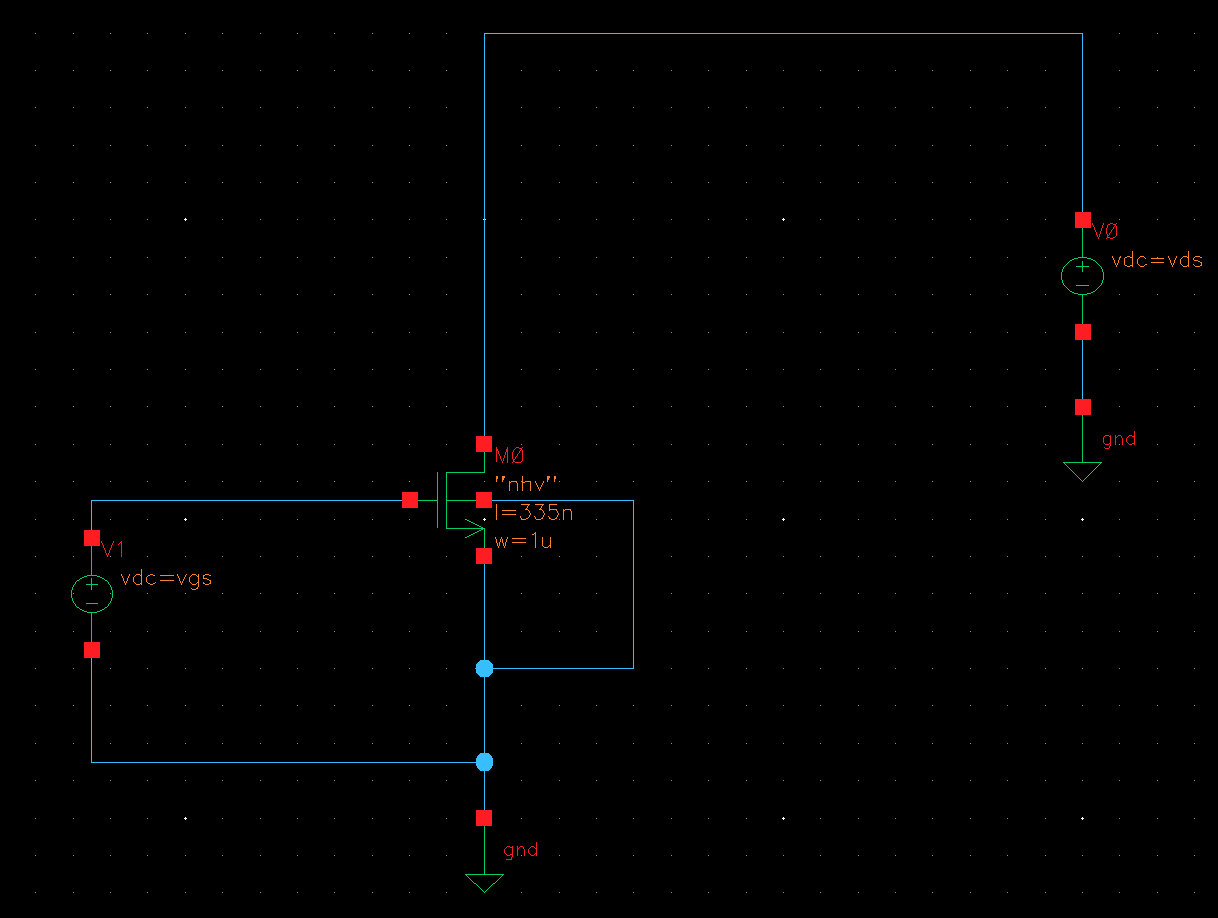
\includegraphics[width=0.9\textwidth]{images/nmos-circuit.png}
	\caption{NMOS Analysis Circuit}
	\label{fig:nmos-circuit}
\end{figure}

The next step was to perform a DC analysis of the circuit. The DC analysis was performed by sweeping the gate voltage ($V_{GS}$) from 0V to 3.3V.
\begin{figure}[h!]
	\centering
	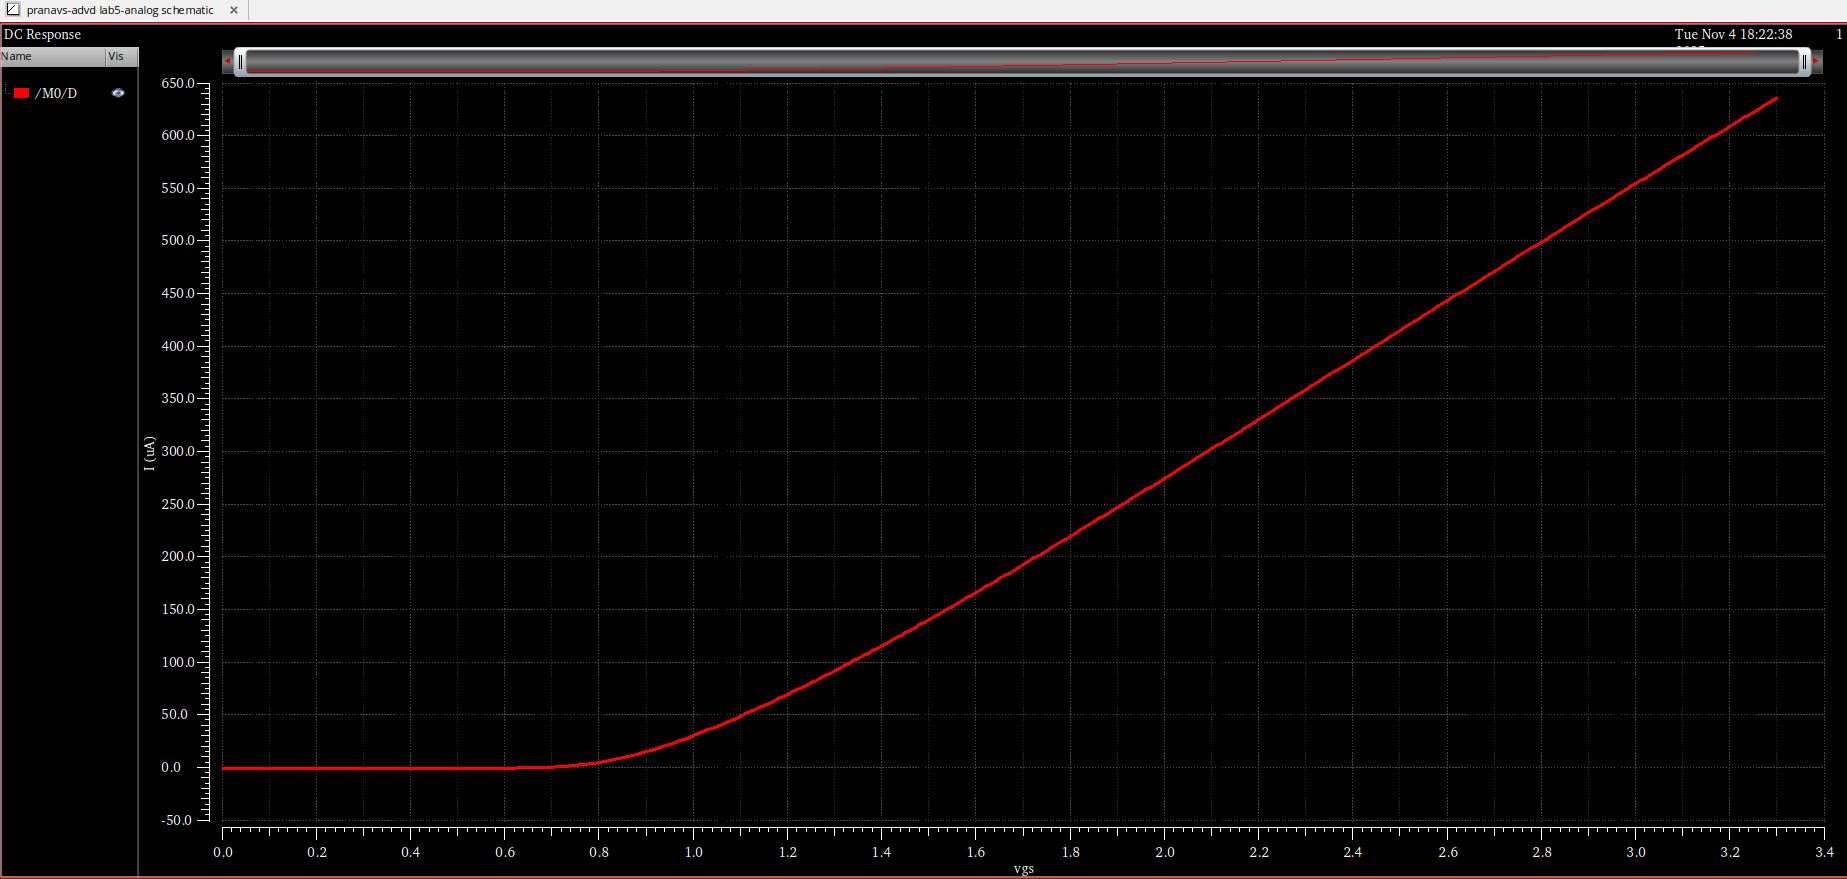
\includegraphics[width=0.9\textwidth]{images/id_vs_vgs.png}
	\caption{$I_D$ vs $V_{GS}$ for NMOS Transistor}
	\label{fig:nmos-dc-analysis}
\end{figure}

The drain voltage ($V_{DS}$) was kept constant at 3.3V. The drain current ($I_D$) was measured for each value of $V_{GS}$. The results of the DC analysis are shown in Figure \ref{fig:nmos-dc-analysis}.

From here, $g_m$ was the next obvous step. $g_m$ was calculated using the formula:
\begin{equation}
	g_m = \frac{dI_D}{dV_{GS}}
\end{equation}
The derivative function in the calculator of Cadence was used in order to produce the $g_m$ vs $V_{GS}$ graph shown in Figure \ref{fig:nmos-gm-analysis}.
\begin{figure}[h!]
	\centering
	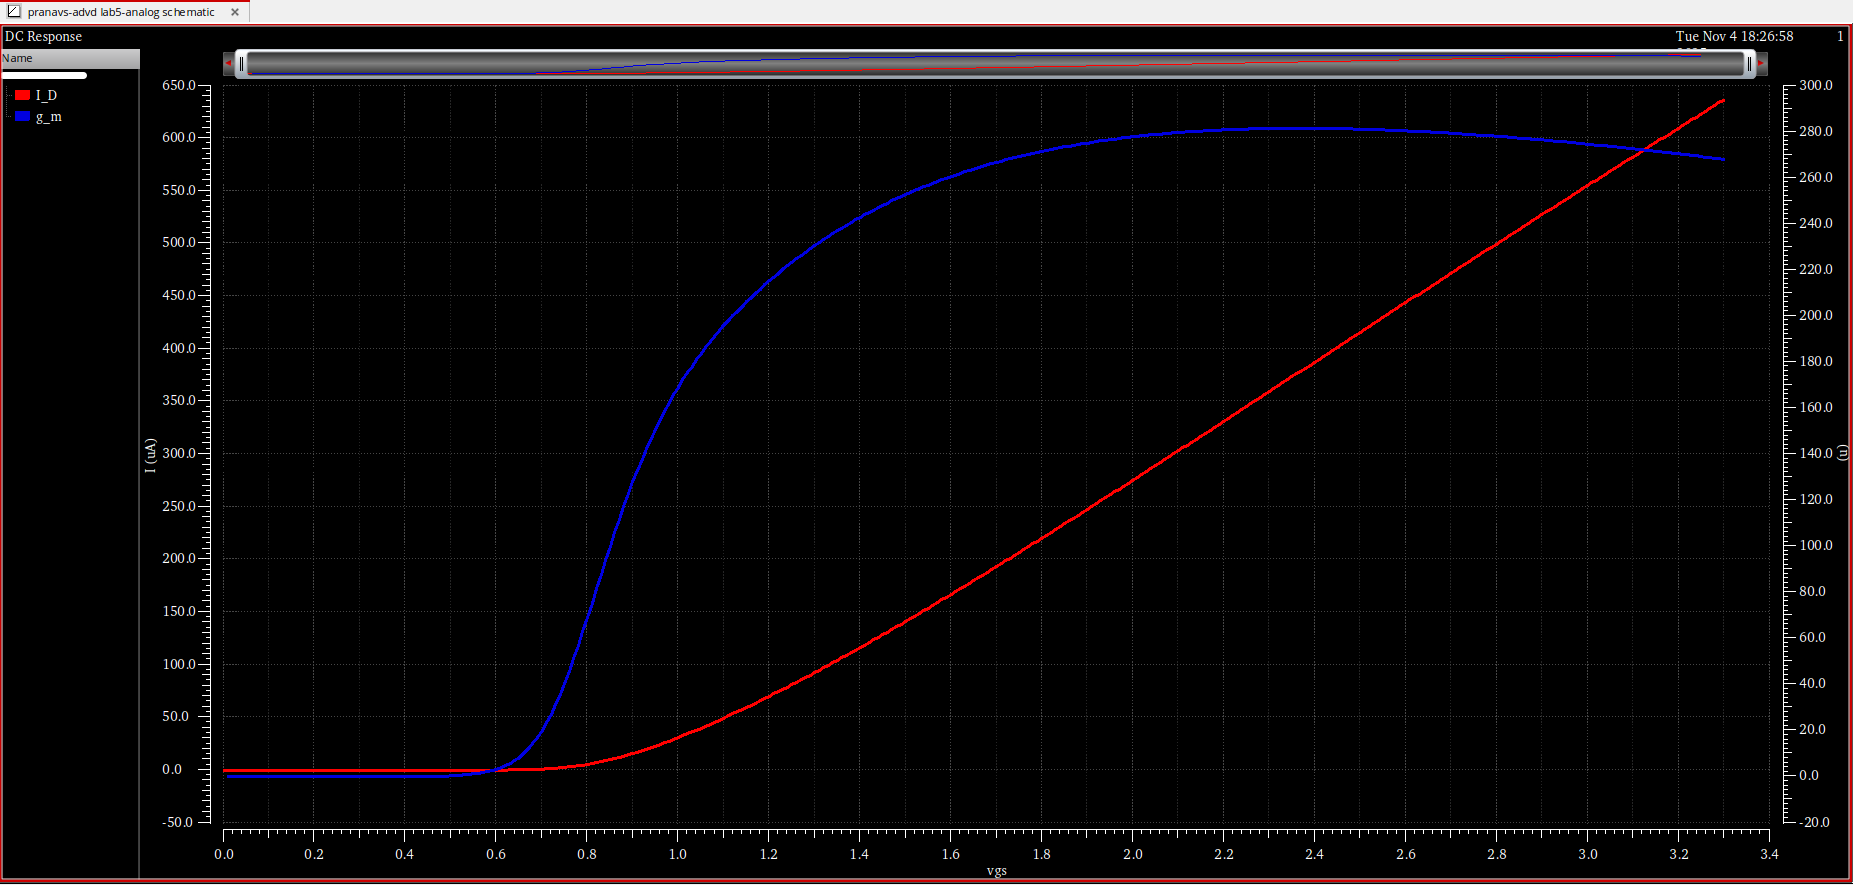
\includegraphics[width=\textwidth]{images/gm_vs_vgs.png}
	\caption{$g_m$ vs $V_{GS}$ (Blue) for NMOS Transistor}
	\label{fig:nmos-gm-analysis}
\end{figure}

Now, the $g_m$ vs $I_D$ graph was plotted using the data from the previous two graphs. The results are shown in Figure \ref{fig:nmos-gm-id-analysis}.
The graph calculator was used in Cadence in order to plot the requisite quantities against each other.
\begin{figure}[h!]
	\centering
	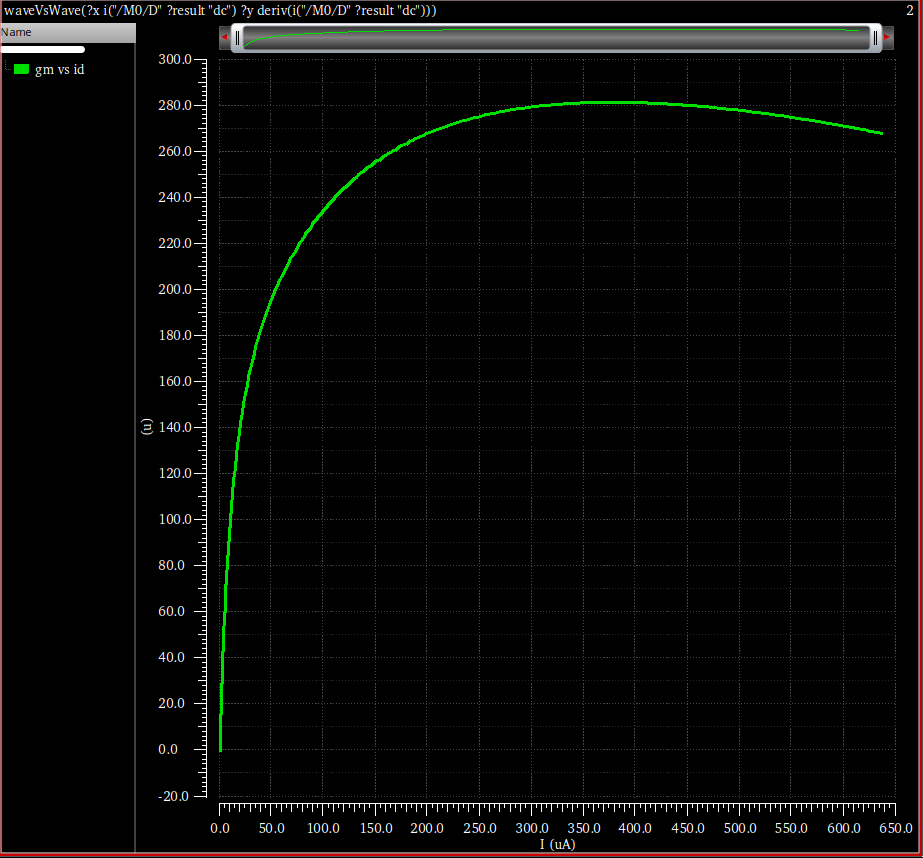
\includegraphics[width=\textwidth]{images/gm_vs_Id.png}
	\caption{$g_m$ vs $I_D$ for NMOS Transistor}
	\label{fig:nmos-gm-id-analysis}
\end{figure}

\clearpage
\section{PMOS Analysis}
The PMOS transistor used for this analysis was the pvh transistor from the Mohali library. The circuit designed in Cadence Virtuoso is shown in Figure \ref{fig:pmos-circuit}.
\begin{figure}[h!]
	\centering
	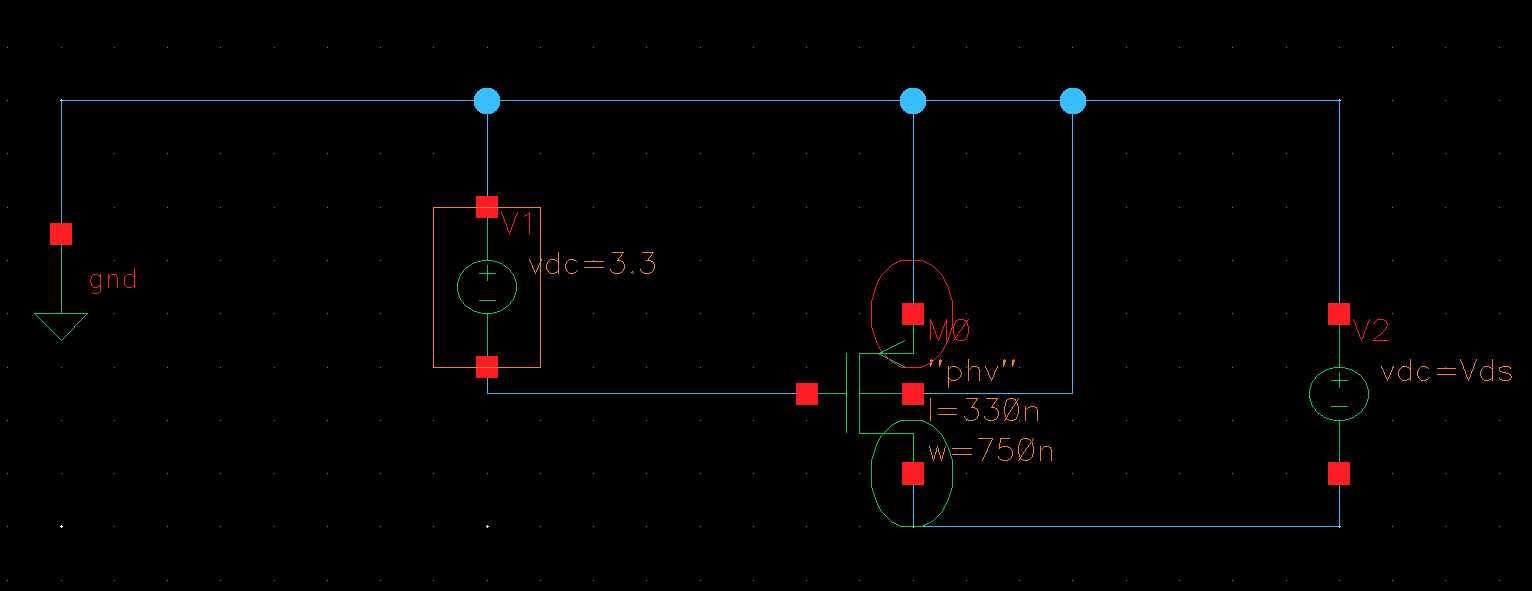
\includegraphics[width=\textwidth]{images/pmos-circuit.png}
	\caption{PMOS Analysis Circuit}
	\label{fig:pmos-circuit}
\end{figure}

The DC analysis was performed by sweeping the gate voltage ($V_{GS}$) from -3.3V to 0V. The drain voltage ($V_{DS}$) was kept constant at -3.3V. The drain current ($I_D$) was measured for each value of $V_{GS}$. The results of the DC analysis are shown in Figure \ref{fig:pmos-dc-analysis}.
\begin{figure}[h!]
	\centering
	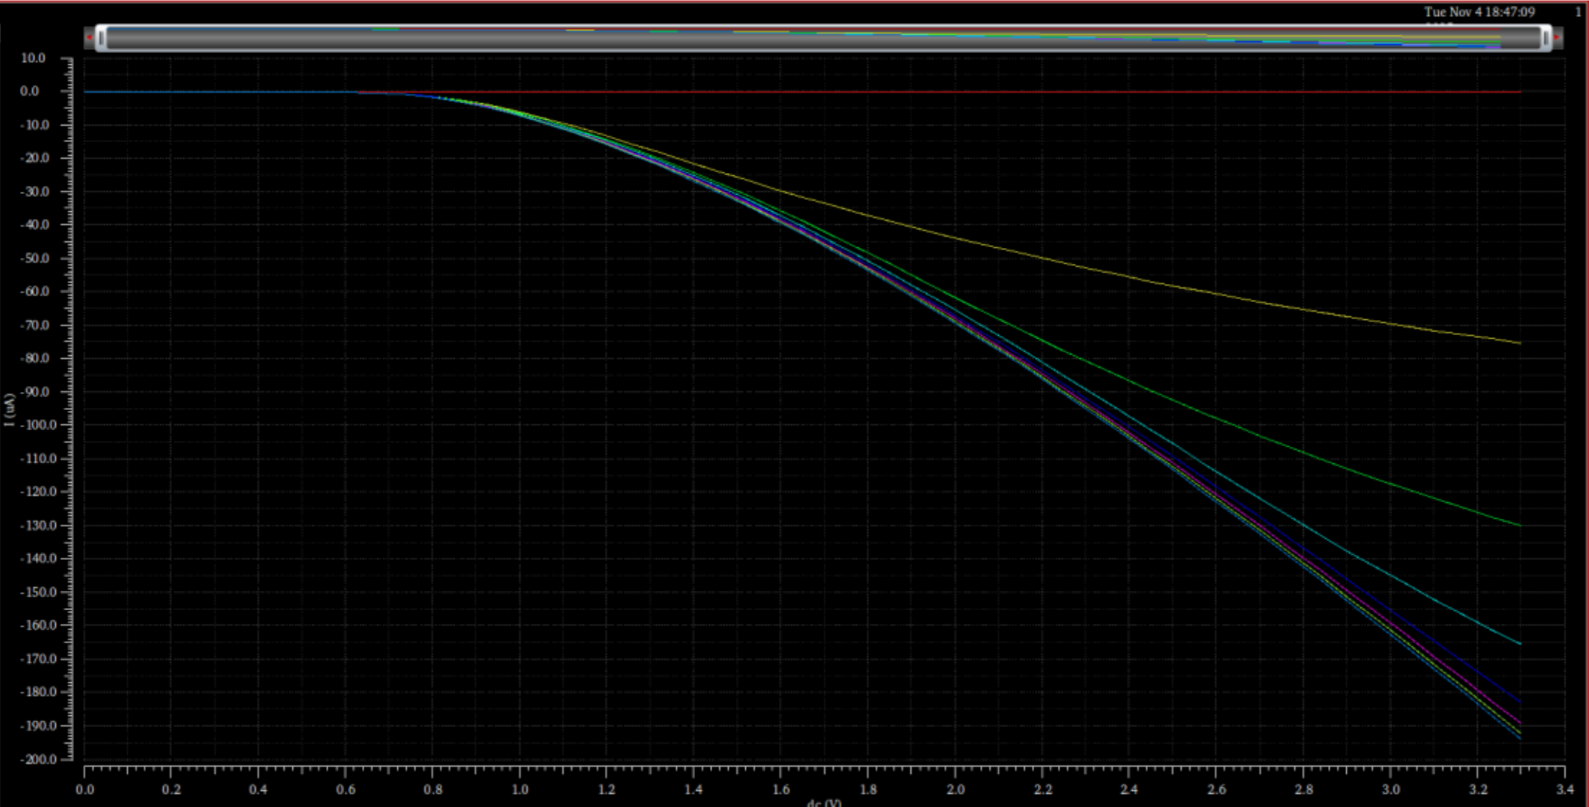
\includegraphics[width=\textwidth]{images/id_vs_vgs_pmos.png}
	\caption{$I_D$ vs $V_{GS}$ for PMOS Transistor}
	\label{fig:pmos-dc-analysis}
\end{figure}

From here, $g_m$ was calculated using the formula:
\begin{equation}
	g_m = \frac{dI_D}{dV_{GS}}
\end{equation}
The derivative function in the calculator of Cadence was used in order to produce the $g_m$ vs $V_{GS}$ graph shown in Figure \ref{fig:pmos-gm-analysis}.
\begin{figure}[h!]
	\centering
	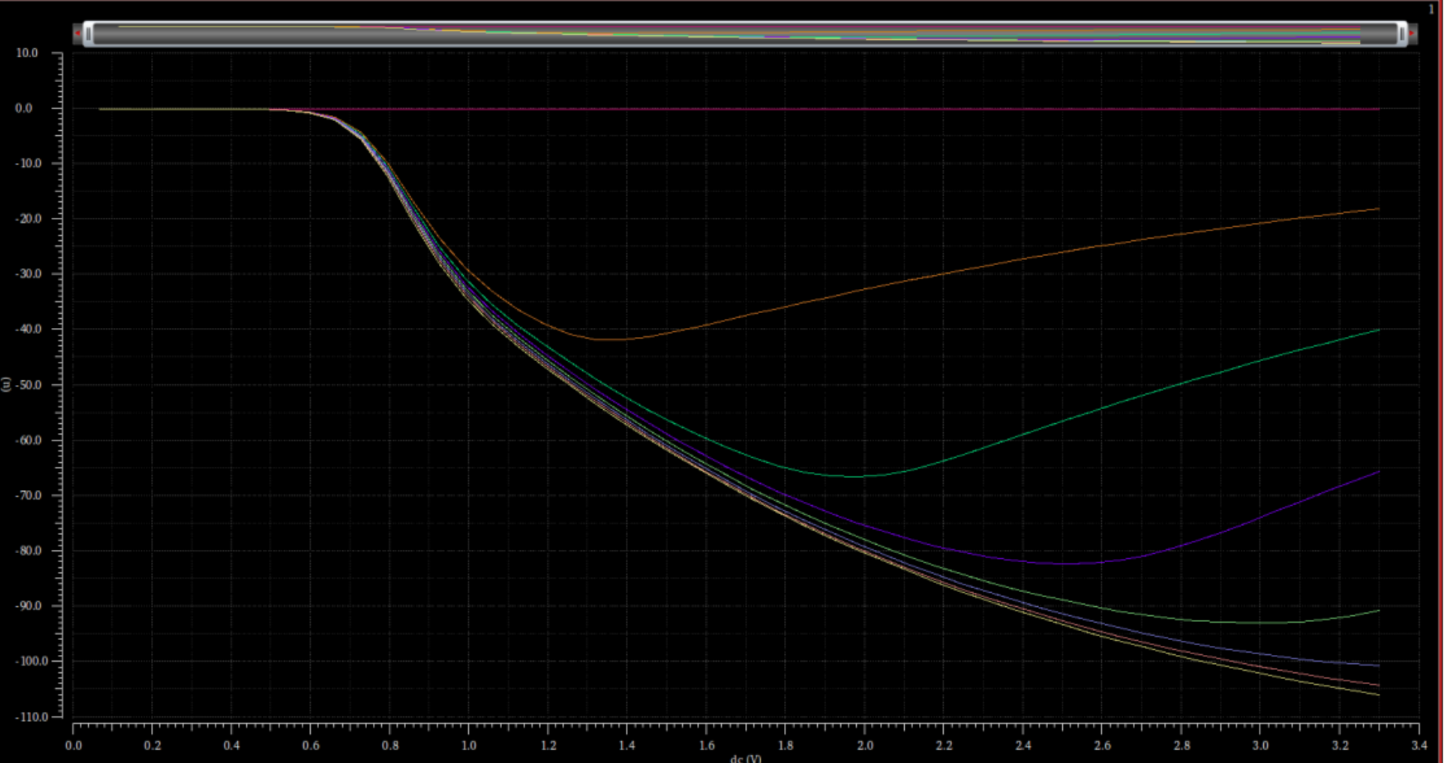
\includegraphics[width=\textwidth]{images/gm_vs_vgs_pmos.png}
	\caption{$g_m$ vs $V_{GS}$ (Blue) for PMOS Transistor}
	\label{fig:pmos-gm-analysis}
\end{figure}

Now, the $g_m$ vs $I_D$ graph was plotted using the data from the previous two graphs. The results are shown in Figure \ref{fig:pmos-gm-id-analysis}.
The graph calculator was used in Cadence in order to plot the requisite quantities against each other.
\begin{figure}[h!]
	\centering
	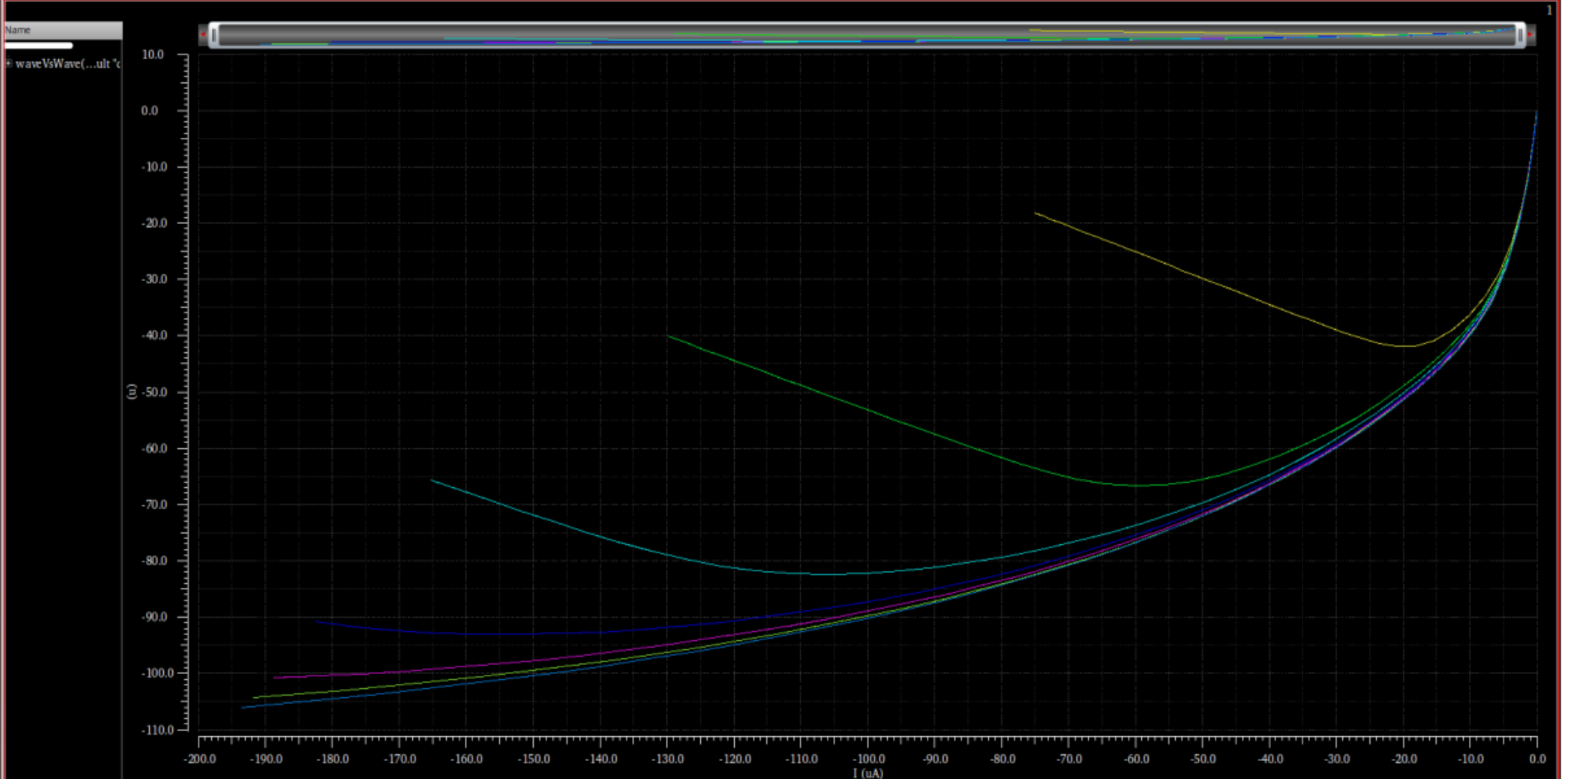
\includegraphics[width=\textwidth]{images/gm_vs_Id_pmos.png}
	\caption{$g_m$ vs $I_D$ for PMOS Transistor}
	\label{fig:pmos-gm-id-analysis}
\end{figure}

\clearpage
\section{Conclusion}
In this lab, we successfully analyzed the characteristics of both NMOS and PMOS transistors using Cadence Virtuoso. We plotted the $I_D$ vs $V_{GS}$ curves and calculated the transconductance ($g_m$) for both types of transistors. The results obtained from the simulations were consistent with the theoretical expectations, demonstrating the fundamental behavior of MOSFETs in analog circuits. This lab provided a solid foundation for understanding transistor operation and will be beneficial for future analog design tasks.

\end{document}

